%% ================================================================================
\chapter{Theory}
\label{ch:theory}
%% ================================================================================
%The theory chapter. These are references \cite{aPaper}, \cite{aThesis}, \cite{aWiki}. Figure \ref{fig:dummy} shows a placeholder. 
%
%\begin{figure}
%  \centering
%  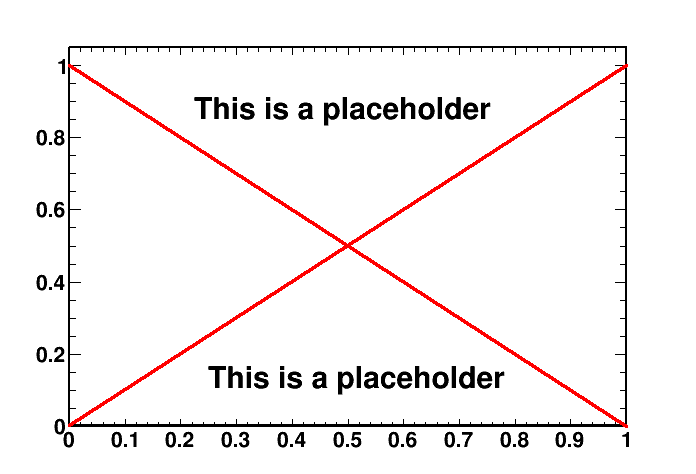
\includegraphics[width=.9\linewidth]{pic/dummy.png}
%  \caption{This is a dummy plot.}
%  \label{fig:dummy}
%\end{figure}
%
%\section{A section}
%\label{sec:section}
%Here we have Section \ref{sec:section}. \todo{This is a TODO marker} You might need this.

\section{Our Milky Way}

\subsection{General properties}


\begin{figure}[h]
  \centering
  \begin{minipage}[h]{0.45\textwidth}
  	\centering
	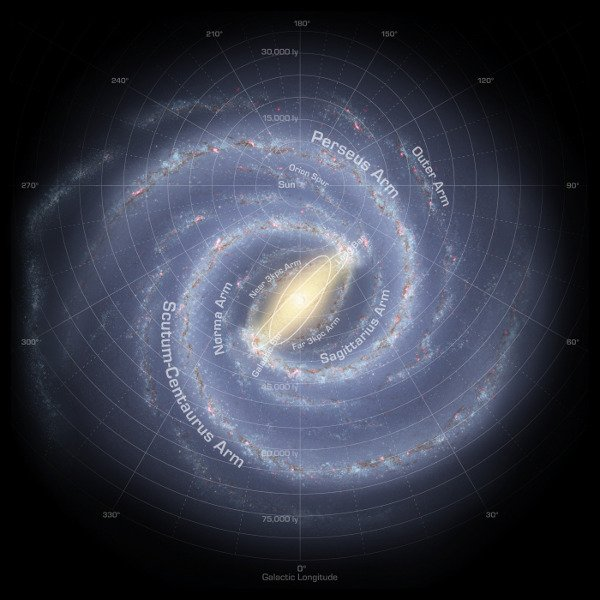
\includegraphics[width=1.\linewidth]{pic/theory/top_galaxy_map.jpg}
  	\subcaption{source: http://galaxymap.org/drupal/node/171}
  	\label{fig:top_gal_map}
  \end{minipage}
  \hfill
  \begin{minipage}[h]{0.45\textwidth}
	  \centering
	  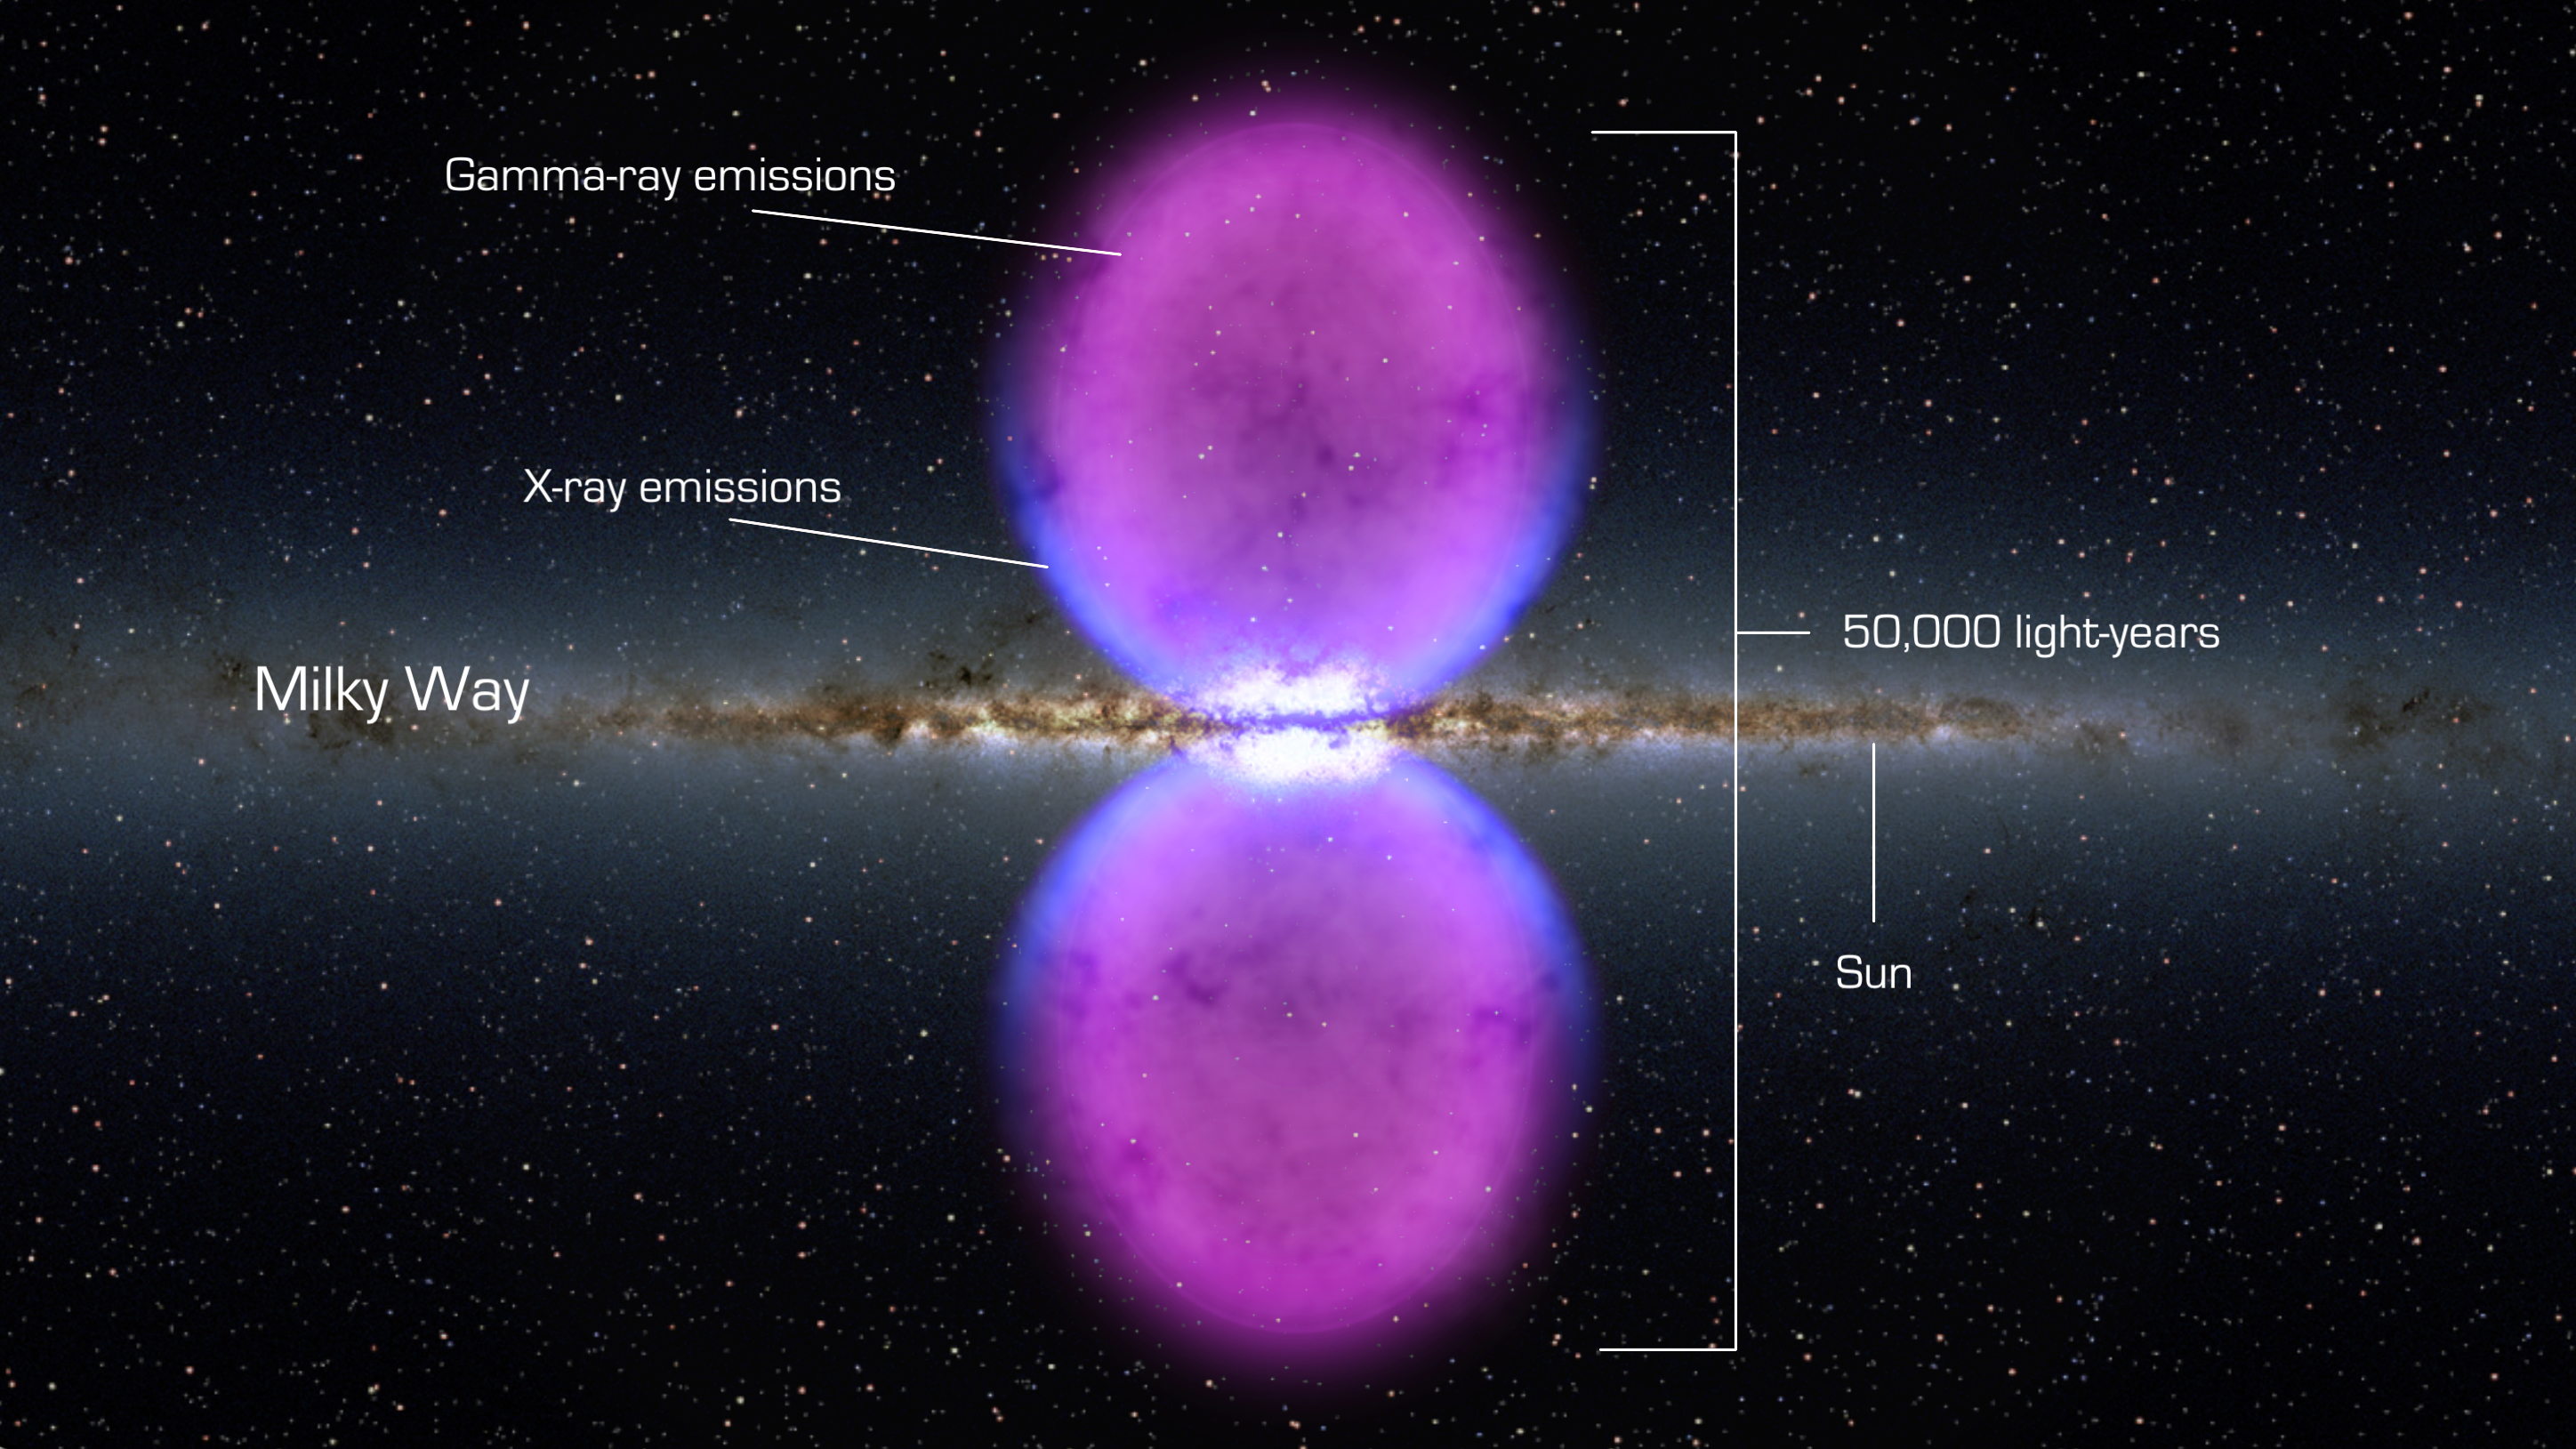
\includegraphics[width=1.\linewidth]{pic/theory/Fermi_bubble.jpg}
	  \subcaption{source: NASA's Goddard Space Flight Center}
	  \label{fig:fermi_bubbles}
  \end{minipage}
  \caption{The Milky Way, as seen from two different angles. }
  \label{fig:Galaxy_maps} 
\end{figure}

For a long time, people thought the universe was constituted only by one galaxy, the Milky Way, the one in which the Sun and the Earth orbit. The discoveries of other galaxies in the universe came only in the 20's thanks to Edwin Hubble. There is still a lot of unknown  around those objects, but the Milky way is pretty well known and will play a major role in the following chapters. Its shape, density and composition are three main factors playing a role in cosmic ray physics and can not be avoided.

First of all, the Milky Way is a barred spiral arm galaxy, meaning it has two main spiral arms, connected in their center by a straight galactic bar. Those arms and bar have higher matter concentration than the rest due to the way stars orbit around the center. Its diameter exceeds 40 kpc for a mass of around $10^{12} M_\odot$ and a thickness under 1 kpc. The Sun and the Earth are rotating 8 kpc from its center in 240 Myr.
All the different objects of the galaxy can be found in this thin disk of matter, mainly in the spiral arm. It includes the stars, planets and over massive objects, but also all the dust and gas clouds. As seen from the Earth, the disk looks like a narrow band of a few degrees in latitude, but with a very high concentration of gas and dust.
In 2010, two large scale structures were detected to the north and the south of the GC. With a diameter of 7kpc, they extend up to 40 degrees in latitude and 20 in longitude. They are a source of high energy gamma-rays and were detected by the Fermi Large Area Telescope (LAT).


\subsection{Dark Matter}

\begin{figure}[h]
 \centering
 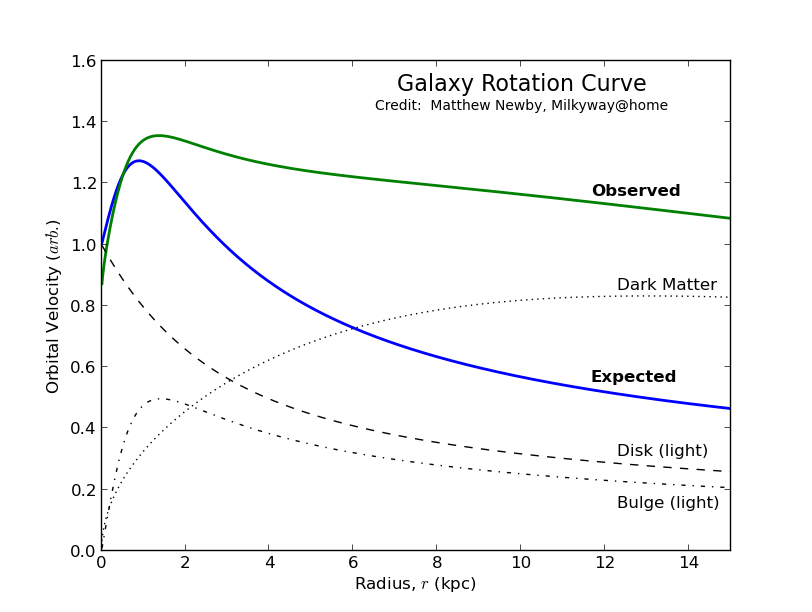
\includegraphics[width=.5\linewidth]{pic/theory/gal_rotation_curve.png}
 \caption{Orbital velocity of the Milky Way as a function of the radius. A clear discrepancy between the theory and the observation can be seen above a 2 kpc radius. Source: Matthew Newby, Milkyway@home}
 \label{fig:gal_rotation_curve}
\end{figure}


The shape of spiral galaxies is well known today, with thousands of examples throughout the universe. This knowledge can be used to mathematically simulate them, and in particular their rotation time as a function of the distance to the center. It was a big surprise when the observed angular speed did not match the theory. One of the solution to explain this difference was the introduction in the standard model of the dark matter (DM), which was suppose to bring a lot of invisible mass into the system. It still has not been observed and a few theories exist on its exact nature. But even without knowing exactly what it is, its mass distribution can still be deduced from the observed rotation curve of the galaxy. The predicted distribution is a spherical halo extending way beyond the 40 kpc of the galactic matter disk. It's density peaks in the GC, and decrease with the radius following a particular density profile. The exact profile is not known, but a popular one is the Navarro-Frenk-White (NFW) profile defined as follows :

\begin{equation}
\rho (r) \propto \frac{1}{\left( r/r_S \right) \left( 1 + r/r_S \right)^2 }
\end{equation}

where $r_S$ is the scale radius.

One of the most popular is the Weakly Interacting Massive Particles (WIMP). They are supposed to be non standard particles with a large mass, neutral, and only sensitive to the weak force, making them very difficult to observe.




\section{Physic of cosmic rays}

\subsection{Creation of CR}
%		-supernovae (SNR)
%		-extra-galactic
%		-pulsars


\subsection{Propagation of CR}
%Propagation through the galaxy
%	-random B field -> no way to backtrace a CR
%	-interaction, shocks in MC
%	-Diffusion coefficient
%		-Can be different in disk, bubbles, or outside
%	-different diffuse coef mean different densities
%		-in MC, bubbles, outside
%		-can observe this inhomogeiniies via gamma rays

Once they are emitted, the cosmic rays propagate through the galaxy under the influence of different interactions.
The first one to notice is the complex manetic field created by all sorts of objects, from the stars to molecular clouds or any distribution of charged particles. It is not particularly strong \todo{put values} compared to the heliosphere or what we can create on Earth, but its very large scale suffice to bend the CR's path in all direction until the point where it is impossible to backtrace its origin.
An other possible interaction is the collisions with other particules. It will obviously depends on the density distribution of those colliders in the galaxy. We can expect a higher number of those in the disk, where the density of molecular clouds the highest.

All these influences can be modeled by a diffusion model, mainly defined by its diffusion coefficient, which discribes the average distance traveled in a certain time. The higher the coefficient, the faster a particule will diffuse in the galaxy. Each phenomenon can be attributed one of those coefficient to describe its effect on the cosmic rays. \todo{give values for Dmag, Dcoll...}
While the diffusion coefficient for the galactic magnetic field can be taken as constant throughout the milky way, the diffusion coefficient due to collision is proportional to the particles density. We can then expect a smaller coefficient in molecular clouds, where the density can reach \todo{value!}.

This coefficient will also define the cosmic ray densities in various locations of the galaxy. Indeed, the more a particle's path is twisted and convoluted, the harder it will be to escape move away from its origin. This way, a higher density of cosmic rays can be found in low diffusion coefficient areas like molecular clouds. In comparison, the region outside the galactic disk has a low density of CR due to a weak magnetic field and small gas and dust density. However, the bubble region is outside the disk and has a higher concentration of CR other regions outside the disk. This is due to a direct outward emission of CR from the GC region in the disk. With a high diffusion coefficient, those CR are ejected light years away \todo{put values}, forming two symetric region extending north and south up to 40 degrees in latitude.


\subsection{Gamma-ray creation}
%		-pion decay
%		-bremmstrahlung
%		-inverse compton

Since the cosmic rays we observe on Earth can not give us a clue about their origin, some indirect detection methods are requiered. Luckily, cosmic rays interact n a lot of ways with their environment, as discribed in the previous section. These interactions can leave detectable traces that can be observed. The most common is the production of light, via creation of high energy photon in the GeV range. Once created, these gamma rays can be blocked or absorbed, but not deflected. Linking the gamma-ray and cosmic ray requires to know the processes in play. Her eis a list of the main phenomena.

\subsubsection{Pion decay}
%Explain phenomenon
%Explain expected gamma ray spectrum, propagated proton distribution.

The high energy protons can produce $\pi^{0}$ which decay almost immediatly in 2 gammas of equal energy.




\subsubsection{Bremmstrahlung}
%Explain phenomenon
%Explain expected gamma ray spectrum


The electrons passing near an other charged particle, or in a magnetic field will be deflected by the electromagnetic interaction. In the process, the electron will lose energy via the emmision of photons. The energy of the latter will depend on the energy of the electron and the intensit of the magnetic ield or the charge of the other particule. The more the electron is deflected, the higher the energy of the emmitted photons.
\todo{give numbers for B field and proton in MC}


\subsubsection{Inverse Compton}
%Explain phenomenon
%Explain expected gamma ray spectrum


A third interaction can link the cosmic ray electrons to gamma rays and it is inverse compton. When a high energy electron collides with a low energy photons, the electron can transfert some of its kinetic energy to the photon, giving him enough energy to enter the gamma range.

So number of gamma rays coming from inverse compton is directly linked tto the electron distribution and the interstellar radiation field (ISRF) of the galaxy. The latter is composed of three major components, the starlight, the dust emission and the cosmological microwave background (CMB). The first component is directly linked to the star distribution, and will be dominant in the disk, where all the star are concentrated. The starlight emits as a blackbody, peaking in the UV range. The dust emission comes from the infra-red emission of warm dust. It will also be mainly present in the disk, since the dust clouds are pretty flat. Finally, the CMB is peaking in the microwave range but is unformely present everywhere in the universe, and therefor in the galaxy. It will be dominant where the two others are negligeable, namely outside the galactic disk.


\todo{talk about synchrotron and ionization losses}

\subsection{Gamma ray observation}

Several instruments in the world observe gamma rays. For example the Fermi Large Area Telescope (LAT) mounted on the ISS. This instrument maps the gamma ray sky between 20MeV and 300GeV \todo{cite}. The diffuse cosmic ray emmision that we are interested in can be obtained after modeling and subtracting the contribution of the over sources. This allows us to compare the observation with the models we obtain from the previous three interactions.



\section{What are the unresolved problems of the precedent chapter}
%What are the unresolved problems of the precedent chapter:
%	-Bad fits in bubbles and disk	
%	-Spherical gamma-ray excess in GC when fitting spatial templates
%		-DM studies
%			-Hooper
%			-others...
%		-MSP studies
%			-Fermi
%			-Hooper
%			-Weniger
%	-High energy tail flux too hard
%	

\begin{figure}
 \centering
 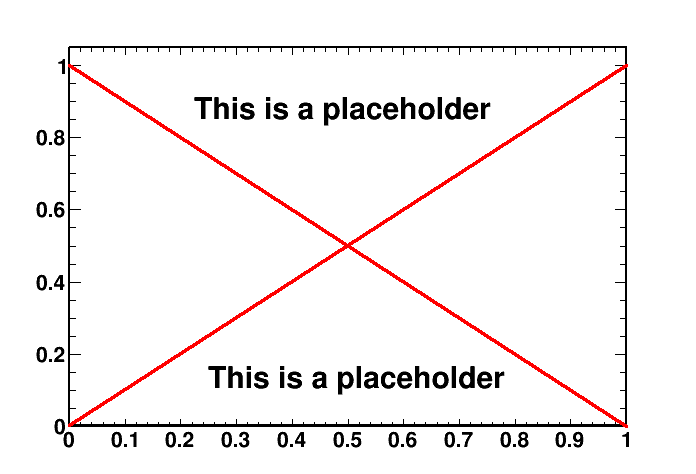
\includegraphics[width=.9\linewidth]{pic/dummy.png}
 \caption{chi2 distribution of first fits (not mines)}
 \label{fig:first_BKGonly_fits}
\end{figure}

Several studies have already tried to see how our predictions of the gamma rays emission and our observations compare. The three main phenomena were modeled as explained to try to recreate the spectrum observed from Earth. The results are clear, there are somethings missing in our interpretation. 
The fit is clearly not working in the galactic plane and the bubbles (as shown on Fig. \ref{fig:first_BKGonly_fits}. The spatial templates used in those fits also show a spherical excess of gamma rays of about 2GeV in the galactic center (GC).

\begin{figure}
 \centering
 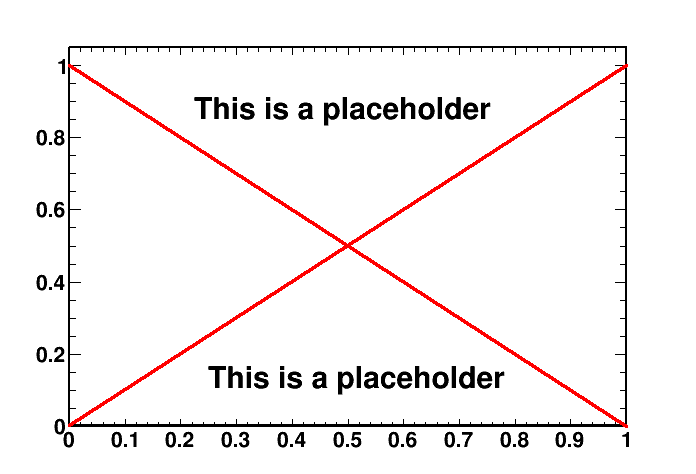
\includegraphics[width=.9\linewidth]{pic/dummy.png}
 \caption{shape of the excess}
 \label{fig:first_BKGonly_fits}
\end{figure}


Two main ideas have emerged to explain this spherical excess.

First is the presence of dark matter in the galaxy in the form of weakly interacting massive particles (WIMP). The spatial distribution of these particles would follow a Navarro-Frrank-White (NFW) profile centered at the GC. They are also expected to produce gamma rays when annihilating with each other via hadrons production. In theory, if the mass of a WIMP particle is around 50GeV, the expected gamma spectrum would peak around 2GeV, where the excess is observed. \todo{cite}
The study of the excess could put strong limits on the mass and annihilation cross section of such WIMP and confirm, or infirm the theory.

The second theory does not involve new physic, but inobserved milli-second pulsars. They would also be spherically distributed around the GC and their gamma spectrum peaks around 2GeV. A few thousands of them would be needed to recreate the intensity of excess. The main default of this explaination resides in the fact that we have observed only a few hundreds? at most. That would requires a very high concentration and a reason why we can not observe them more easely.







































